\clearpage
\slidetitle{Résultats expérimentaux}

\begin{slide}

\begin{itemize}
	\item \textbf{Entrée:} $3\times 5$.
	\item \textbf{Sortie:} chiffres de 0 à 9.
	\item \textbf{Échantillons:} 10 par classe pour l'apprentissage, 1 par classe pour la validation.
\end{itemize}

\begin{figure}[h]
	\centering
	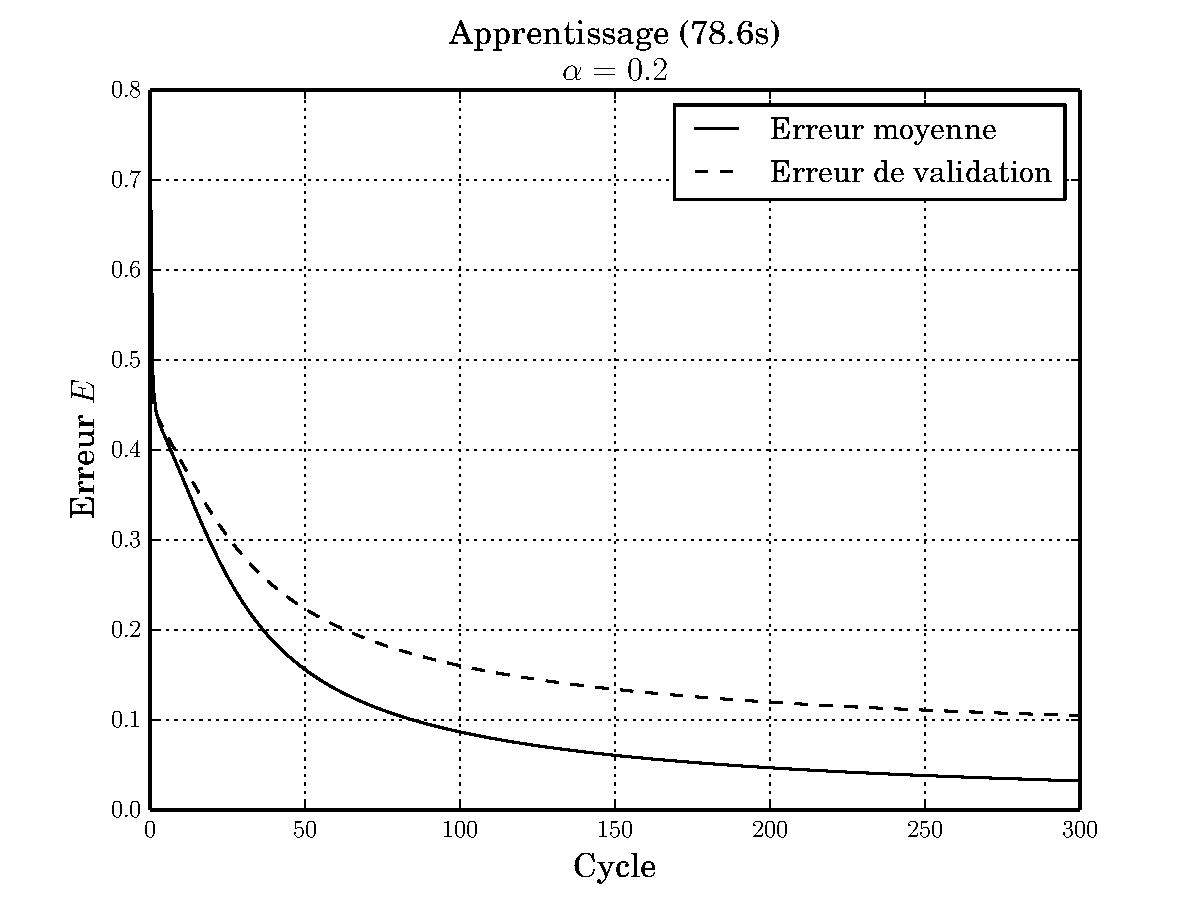
\includegraphics[width=\linewidth]{{graphes/mono_0.2}.pdf}
	\caption*{Monocouche}
\end{figure}

\end{slide}

\clearpage
\slidetitle{Résultats expérimentaux}

\begin{slide}

\begin{figure}[h]
	\centering
	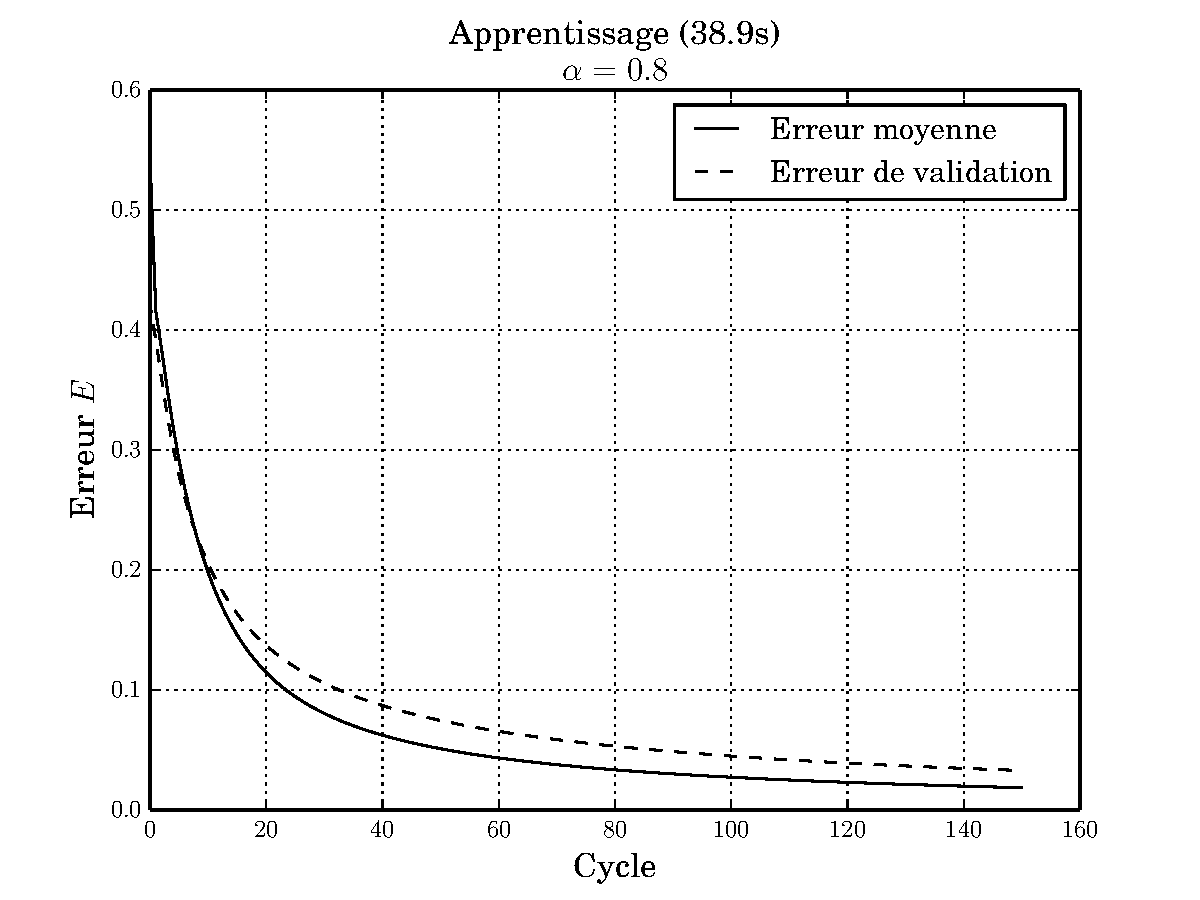
\includegraphics[width=\linewidth]{{graphes/mono_0.8}.pdf}
\end{figure}

\end{slide}

\clearpage
\slidetitle{Résultats expérimentaux}

\begin{slide}

\begin{figure}[h]
	\centering
	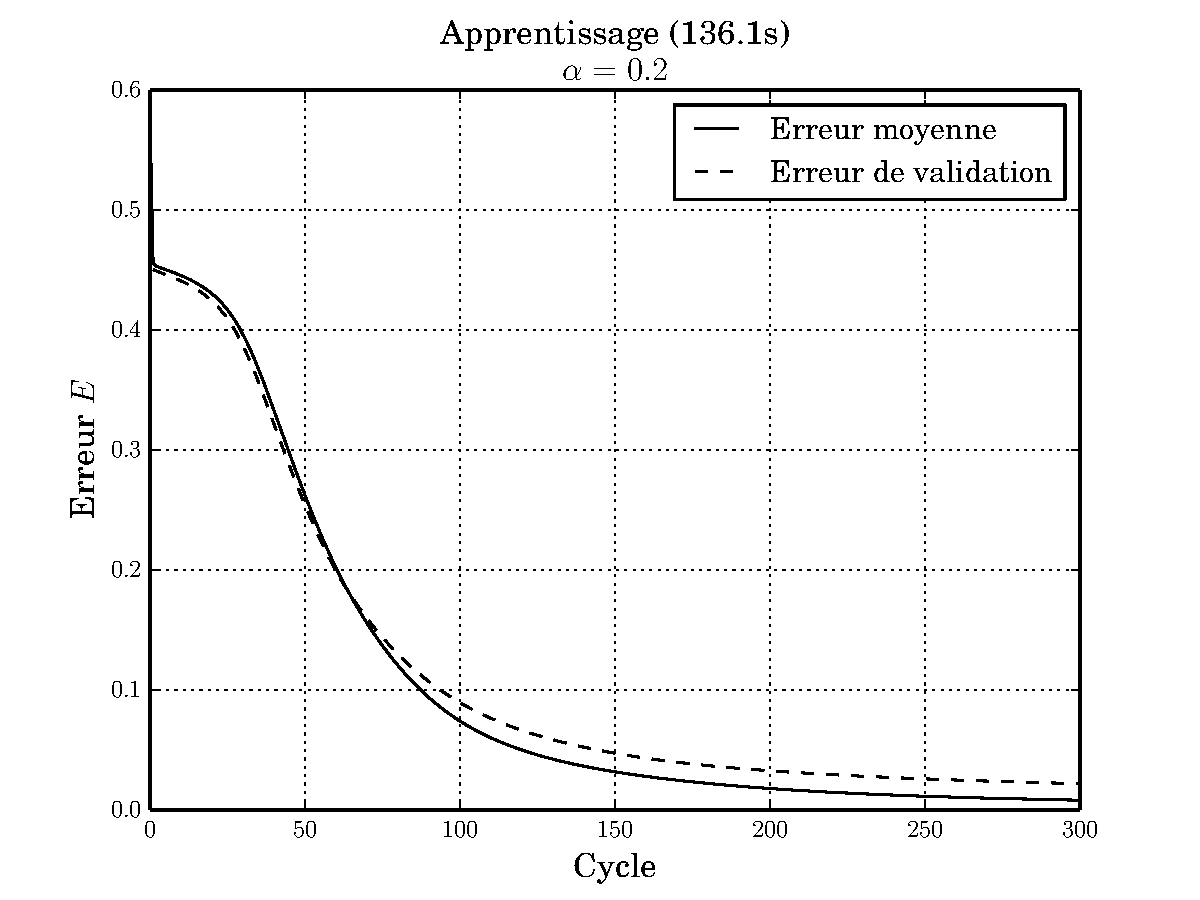
\includegraphics[width=\linewidth]{{graphes/16_0.2}.pdf}
	\caption*{Multicouche (16, 10)}
\end{figure}

\end{slide}

\clearpage
\slidetitle{Résultats expérimentaux}

\begin{slide}

\begin{figure}[h]
	\centering
	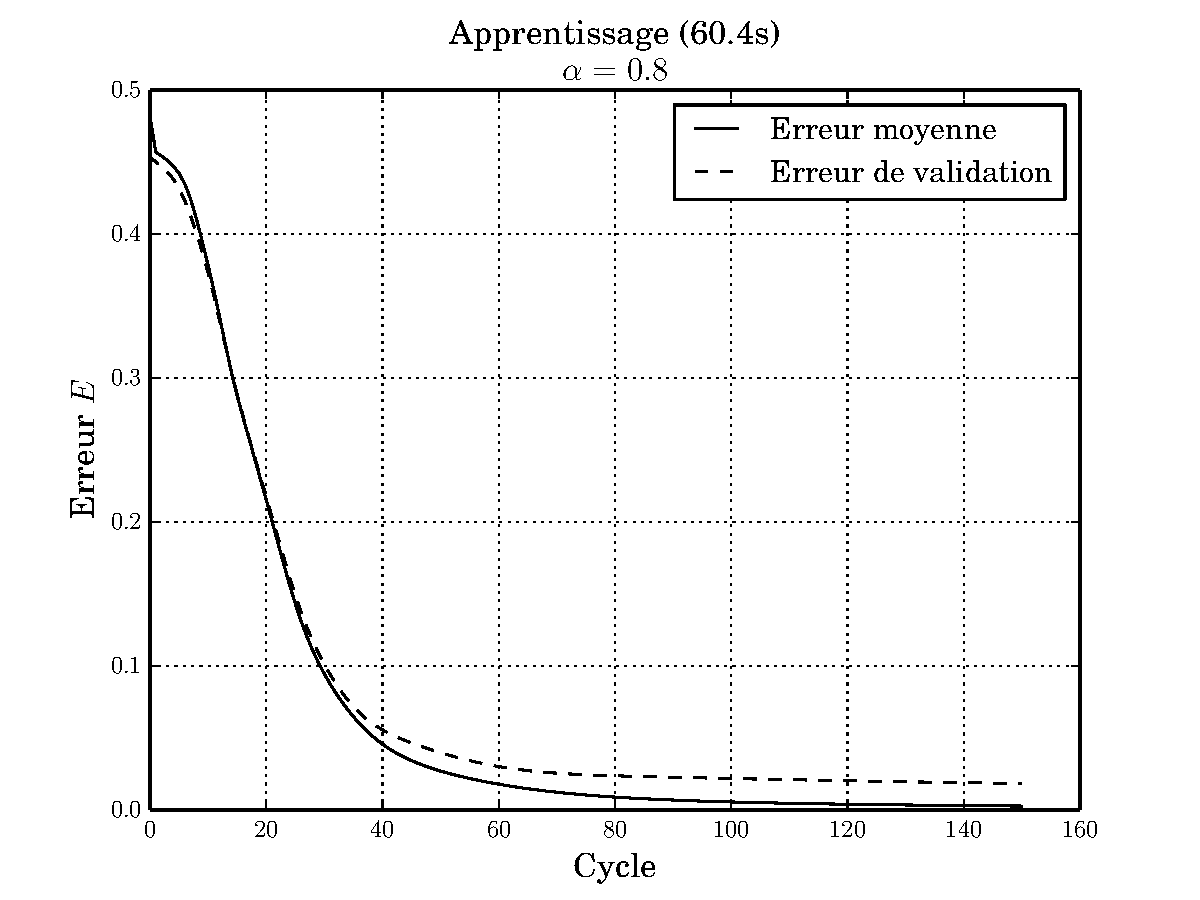
\includegraphics[width=\linewidth]{{graphes/16_0.8}.pdf}
\end{figure}
\end{slide}

\clearpage
\slidetitle{Résultats expérimentaux}

\begin{slide}

\begin{figure}[h]
	\centering
	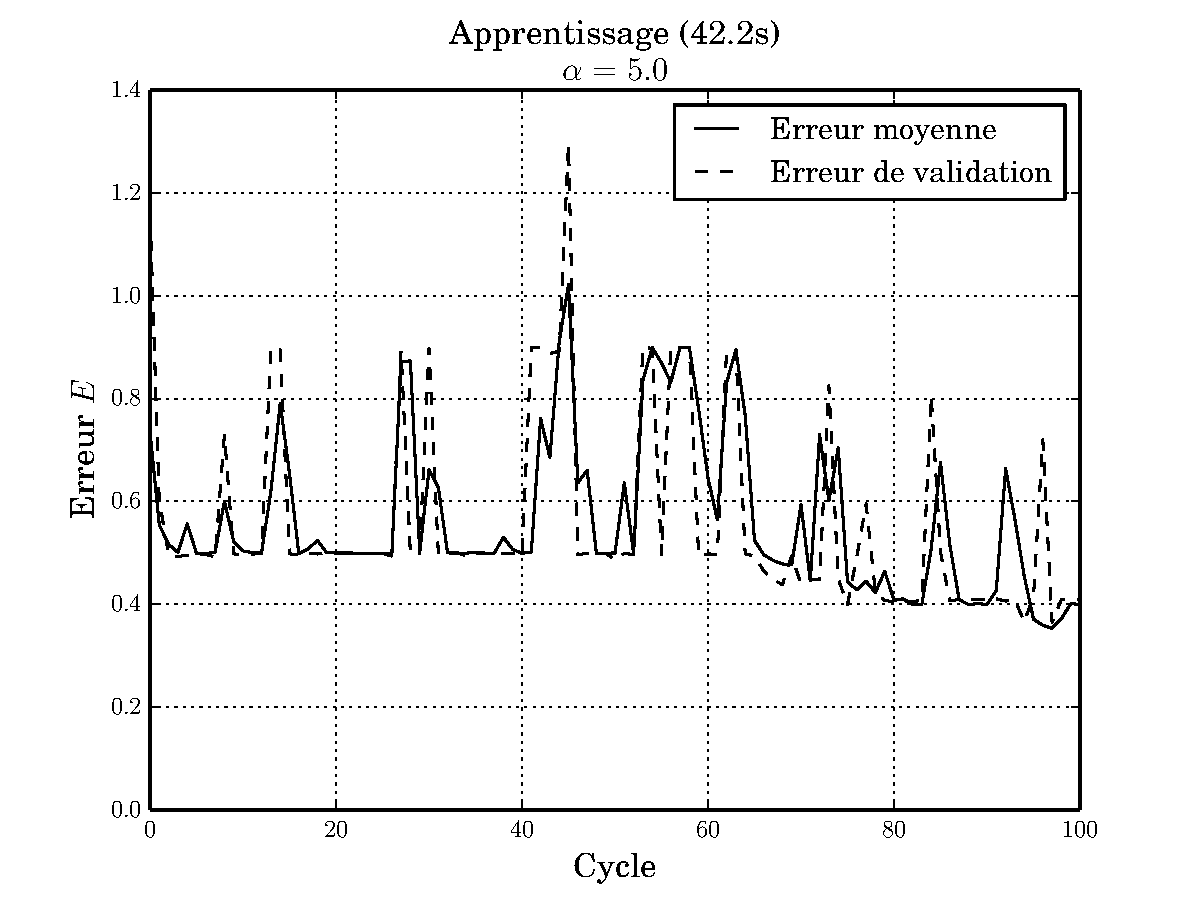
\includegraphics[width=\linewidth]{{graphes/16_5}.pdf}
\end{figure}
\end{slide}

\clearpage
\slidetitle{Résultats expérimentaux}

\begin{slide}

\begin{figure}[h]
	\centering
	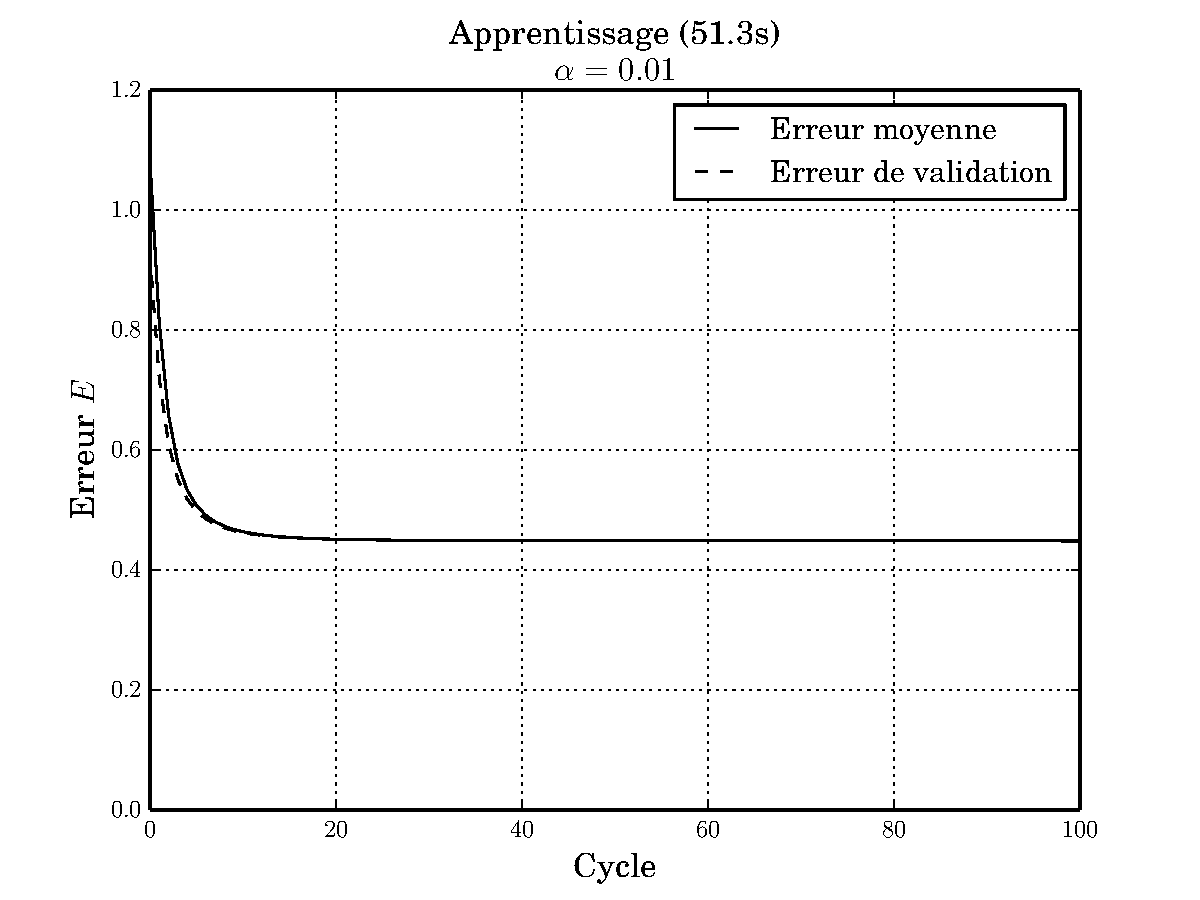
\includegraphics[width=\linewidth]{{graphes/16_12_0.01}.pdf}
	\caption*{Multicouche (16, 12, 10) }
\end{figure}
\end{slide}